\documentclass[tikz]{standalone}

\colorlet{FilledSurface}{blue!20}
\colorlet{FilledSurfaceGroupOne}{blue!20}
\colorlet{FilledSurfaceGroupTwo}{red!20}
\colorlet{FilledSurfaceGroupThree}{green!20}
\colorlet{FilledSurfaceGroupFour}{magenta!20}
\colorlet{FormulaBackground}{green!10}
\colorlet{FormulaFrame}{green}


\usetikzlibrary{intersections}

\begin{document}
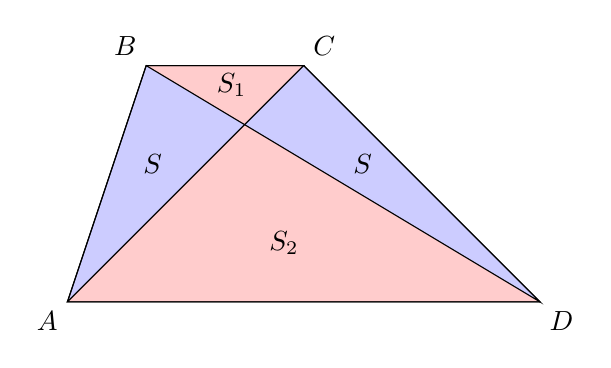
\begin{tikzpicture}

\coordinate (A) at (0, 0);
\coordinate (B) at (1, 3);
\coordinate (C) at (3, 3);
\coordinate (D) at (6, 0);

\draw[name path=BD] (B) -- (D);
\draw[name path=AC] (A) -- (C);

\path [name intersections={of=AC and BD, by=I}];

% Colorear superficies
\fill[FilledSurfaceGroupOne] (A) -- (B) -- (I);
\fill[FilledSurfaceGroupOne] (C) -- (D) -- (I);
\fill[FilledSurfaceGroupTwo] (B) -- (C) -- (I);
\fill[FilledSurfaceGroupTwo] (D) -- (A) -- (I);

\node at (barycentric cs:A=1,B=1,I=1) {$S$};
\node at (barycentric cs:B=1,C=1,I=1) {$S_1$};
\node at (barycentric cs:C=1,D=1,I=1) {$S$};
\node at (barycentric cs:D=1,A=1,I=1) {$S_2$};

% Dibujamos los segmentos, luego de colorear las superficies para
% evitar que las superficies cubran a los segmentos.
\draw
(A) node [below left] {$A$}
-- (B) node [above left] {$B$}
-- (C) node [above right] {$C$}
-- (D) node [below right] {$D$}
-- cycle;
\draw (A) -- (B) -- (I);
\draw (C) -- (D) -- (I);
\draw (B) -- (C) -- (I);
\draw (D) -- (A) -- (I);

\end{tikzpicture}
\end{document}
